\documentclass[
% opciók nélkül: egyoldalas nyomtatás, elektronikus verzió (fekete linkek)
% twoside,     % kétoldalas nyomtatás
% colorlinks,  % elektronikus verzió (színes linkek)
% tocnopagenum,% oldalszámozás a tartalomjegyzék után kezdődik
]{thesis-ekf}
\usepackage[T1]{fontenc}
\PassOptionsToPackage{defaults=hu-min}{magyar.ldf}
\usepackage[magyar]{babel}
\footnotestyle{rule=fourth}
\usepackage{natbib}
\usepackage{listings,xcolor}
\setcitestyle{aysep={}}

\begin{document}
\institute{Matematikai és Informatikai Intézet}
\title{Középiskolai e-napló fejlesztése MVC keretrendszer használatával}
\author{Renyhárt Gábor\\programtervező informatikus BSc}
\supervisor{Balla Tamás\\tanársegéd}
\city{Eger}
\date{2020}
\maketitle

\tableofcontents

\chapter*{Bevezetés}
Mindannyian voltunk diákok, jártunk iskolába, és mindenki kapott jegyet. Az én időmben még papír alapon. A naplóba, amitől mindig féltünk feleléskor, hogy hol nyílik ki. Már általános iskola végén sem értettem, hogy ha ennyi számítógép van már a világban, akkor miért nem használják egy ilyen területen, ahol sok az adminisztráció, és sok a hibázási lehetőség.

Erre lett megoldás Magyarországon a 2018 szeptemberében kötelezővé tett e-napló használata az iskolákban. Korábban már több intézmény használt saját fejlesztésű, vagy egy vállalat által elkészített elektronikus naplót.

A Digitnaplo Kft. által fejlesztett IEAR (Iskolai Elektronikus Adminisztrációs Rendszer) felkerült az Educatio Nonprofit Kft által összeállított azon programok listájára, melyeket az oktatási intézmények hivatalosan használhatnak (2016 szeptember).

A Mozaik Kiadó által kifejlesztett elektronikus napló, a mozaNapló lehetővé teszi az iskola mindennapjai során felmerülő adatkezelési, szervezési és statisztikai feladatok számítógéppel történő elvégzését. A digitális napló alkalmazásával feleslegessé válik a hagyományos papíralapú naplók vezetése és jelentősen csökkenti a pedagógusok adminisztrációs terheit. Minden internetkapcsolattal rendelkező számítógépről elérhető, nem szükséges külön programot telepíteni. Használatához mindössze alapfokú internetkezelési ismeretek szükségesek.

A Neptun KRÉTA (Köznevelési Regisztrációs és Tanulmányi Alaprendszer) a továbbiakban KRÉTA a köznevelési intézmények oktatásszervezői feladatait támogató informatikai rendszer, amely a köznevelés más rendszereivel integráltan és adaptívan együttműködik. 

Az évek során a tanulmányaim folytán jutottam el arra a szintre, hogy képes vagyok egy ilyen alkalmazás megírására. A programom elkészítése során megvizsgáltam a fentebb említett különböző rendszerek működését, funkcióit, előnyeit. Olvastam véleményeket, és ez alapján állítottam össze a saját követeleménylistámat az én e-naplómmal kapcsolatban.
Ki tudja, esetleg pont ez az alkalmazás lesz a jövő középiskolai elektronikus rendszerének az alapja.


\chapter{Probléma kifejtése}
A jelenleg használatban lévő e-naplók a vélemények szerint bonyolultak, sok időt vesznek el az oktatóktól, az adminisztrátoroktól, és a diákoknak sem esik kézre. Viszont nincsenek olyannyira kihasználva, amennyire a XXI. századi felhasználóknak szüksége lenne rá. A célom, hogy egy olyan alkalmazást készítsek el, ami kellően egyszerűen, gyorsan használható és szinte tökéletes. Csak szinte, hiszen mindig lesznek olyan dolgok, amiket egyszerűbben nem lehet megoldani, csak ha máshonnan veszünk el erőforrást. Azaz ha egy funkció egyszerűbb a felhasználónak, az a feldolgozó rendszernek bizonyosan bonyolultabb. Tovább tarthat az adatok kinyerése az adatbázisból, valamint a megjelenítés is tovább tarthat, ami több -- azaz néhány száz vagy akár ezer felhasználónál -- már jelentős lassúsággal járna.\\
A fejlesztés során folyamatosan konzultáltam tanár szakos hallgatókkal, akik ismerik a jelenlegi helyzetet, és egyes dolgokat meg tudnak közelíteni más módokon is. Több tíz éve a pályán lévő tapasztalt pedagógusok véleményét is kikérdeztem, hiszen ők a régebbi papír alapú rendszert is használták, és ezt az új e-rendszerben is benne vannak.
\chapter{Implementálás}
A programot PHP nyelven írtam, a Codeigniter keretrendszer segítségével. Néhány helyen alkalmaztam Javascriptet a felhasználói élmény fokozása érdekében. A megjelenítésért pedig a Bootstrap a felelős. A kódot a Sublime Text 3 programmal írtam. A saját rendszeremen a WAMP alkamazás szolgáltatásait használtam.
\section{Codeigniter}
A Codeigniter használata egyszerű, könnyen lehet teljes értékű web alkalmazásokat fejleszteni vele. A jelenlegi stabil kiadása a 4.0.4 verzió, amit 2020. július 15-én adtak ki. A szakdolgozati programom elkészítésének a kezdetén még a 3-as verzió volt a legújabb, így azzal a verzióval haladtam a végéig.
A Codeigniter egy nagyon hatékony, mégis kevés memóriát és lemezterületet használó PHP keretrendszer. Az MVC tervezési mintát használja, amelynek lényege, hogy a sok adatot a felhasználó elé táró számítógépes alkalmazásokban az adathoz (modell) és a felhasználói felülethez (nézet) tartozó dolgok szétválasztódjanak azért, hogy a felhasználói felület ne befolyásolja az adatkezelést, és az adatok átszervezhetők legyenek a felhasználói felület változtatása nélkül. Ezt az elképzelést a Codeigniter egy controller közbeiktatásával éri el.

Működése a következő:\\
Egy weboldal betöltése a megfelelő controller megfelelő metódusával kezdődik. 
\lstset{language=php,basicstyle=\footnotesize\ttfamily,
	keywordstyle=\color{blue},
	stringstyle=\color{red},
	identifierstyle=\color{black},
	emph            =[1]{Welcome,CI_Controller,index,\$data,get_news},
	emphstyle       =[1]\color{blue},
	numbers=left,frame=r}
\begin{lstlisting}
class Welcome extends CI_Controller
{
	public function index()
	{
		$data['news'] = $this->news_model->get_news();
		$this->load->view('news/index', $data);
	}
}
\end{lstlisting}
\newpage
Ez a programrészlet hozzáfér az adatbázishoz a modellen keresztül. A modellben valamilyen adatbáziskezelői parancs fut le. Úgymint lekérdezés, beszúrás, törlés, módosítás. 
\lstset{language=php,basicstyle=\footnotesize\ttfamily,
	keywordstyle=\color{blue},
	stringstyle=\color{red},
	identifierstyle=\color{black},
	emph            =[1]{get_news,\$query,News_model,CI_Model},
	emphstyle       =[1]\color{blue},
	numbers=left,frame=r}
\begin{lstlisting}
class News_model extends CI_Model
{
	public function get_news()
	{
		$query = $this->db->get('news');
		return $query->result_array();
	}
}
\end{lstlisting}
A parancs lefutása után a vezérlés -- lekérdezés esetében a lekérdezett adattal együtt -- a controllerbe kerül vissza, amely előkészíti az adatokat a view számára, majd meghívja a viewt, ami a 7.sor alapján a news/index helyen található, majd a \$data változón keresztül hozzákapcsolja a szükséges adatokat. Amint a view megkapta az adatokat, megjeleníti azokat, és kezdődik minden elölről, a felhasználó interakciója alapján.
\section{Javascript}
A Javascriptet 1995-ben hozták létre, az akkori statikus weboldalak fejlesztéséért.
Több paradigmás nyelvként a Javascript támogatja az eseményvezérelt, a funkcionális és az imperatív programozási stílusokat. Alkalmazásprogramozási interfészekkel (API) rendelkezik a szöveggel, dátummal, reguláris kifejezésekkel, adatstruktúrákkal való munkához. Magának a nyelvnek nincs be-kiírató funkciója, ezeket a feladatokat a gazda környezet, általában egy web böngésző biztosítja.
\section{Bootstrap}
A Bootstrap egy nyílt forrású webes keretrendszer, ami az informatív weboldalak fejlesztésének leegyszerűsítésére fókuszál. Az elsődleges célja, hogy ezt egy webprojekthez adjuk, az nem más, mint megkaphassuk a Bootstrap választásait a színek, méretek, betűtípusok, és kinézetek tekintetében.  Amint egy projekthez hozzáadjuk, a Bootstrap biztosítja az alap stílus meghatározásokat minden HTML elem számára. Az eredmény egy egységes megjelenés a táblák, és űrlap elemek megjelenésének miden webböngészőben
A legelső változatot 2011. augusztus 19-én adták ki, miután átnevezték a projektet Twitter Blueprintről. A Bootstrap 2 2012 januárjában jelent meg, a 3-as verzió pedig 2013 nyarán. A 4. kiadást 2018 elején véglegesítették. A Bootstrap 5 Alfa verziója 2020 nyarán jelent meg.
\section{Sublime Text 3}
A Sublime Text egy shareware többplatformú forráskód szerkesztő. Számos programozási és jelölő nyelvet támogat. Pluginek segítségével a felhasználók funkciókat adhatnak hozzá.
\section{WAMP}
A WAMP egy Windowson futtatható alkalmazáskiszolgáló programcsomag, amely fő elemeit az alábbi négy program alkotja:
\begin{itemize}
	\item Windows, a Microsoft által gyártott operációs rendszer.
	\item Apache HTTP Server, egy szabad szoftver/nyílt forrású webszerver, jelenleg a legnépszerűbb.
	\item MySQL, egy többszálas, többfelhasználós SQL adatbázis-kezelő rendszer (DBMS), a Sun Microsystems tulajdonában, több mint 11 millió installációval.
	\item PHP (PHP: Hypertext Preprocessor), egy programozási nyelv, amit eredetileg dinamikus weboldalak fejlesztésére terveztek. A PHP-t leggyakrabban szerveroldali alkalmazásoknál használják, de parancssorból/konzol alól is használható.
\end{itemize}

\section{Az adatbázis}
 Az adatbázisban az adattáblák harmadik normálformában vannak, 19 tábla összekapcsolásából áll össze az alkalmazás.
 Néhány tábla szerkezete:

 users: A program felhasználóinak adatait tárolja. A személyes adatai mellett a diákok esetében az osztályát, és minden felhasználónak a beosztását.
 
 jegyek: A diákok jegyeit tartalmazza. A tábla tartalmazza természetesen a diák azonosítóját, a jegy adóját, azaz a tanár azonosítóját. Az jegy adásának időpontját másodperc pontossággal, magát a jegyet, és hogy melyik tárgyból kapta az érdemjegyet. Két mező van arra, hogy egy jegyhez tartozó dolgozatot lehessen hozzáfűzni, és egy van arra, hogy a diák dolgozatát lehessen ide feltölteni.
 
 haladasi\_naplo: A tanárok ebbe a táblába töltik fel azt, hogy melyik órán mit csinálnak, illetve mit fognak csinálni. A tantárgy azonosítóját természetesen tartalmazza, emellett az adott tantárgy, adott osztályában lévő óra sorszámát, az aznapi óra dátumát, és természetesen a tevékenységet, hogy azon a napon mi történik.
 
 users\_sets: A felhasználók által választható az oldal megjelenítése bizonyos funkcióknál. Ebben a táblában ez kerül eltárolásra. A felhasználó azonosítója természetesen itt van, aztán a set\_name mezőben tárolom azt, hogy melyik kinézetről van szó. Például az 'ofonezet' beállítás az osztályfőnöknek azt a beállítását tartalmazza, hogy a saját osztályának a jegyeit vagy a hiányzását jelenítse meg. Maga a beállítás értéke pedig -1-et, illetve 1-et vehet fel. A program ez alapján eldönti, hogy mely kinézetet kell megjelenítenie.
 
 szulogyermek: Ebben a táblában kerülnek összekapcsolásra a szülők a gyermekeikkel. El van tárolva a szülő azonosítója, a gyermek azonosítója, valamint egy harmadik mezőben, amelynek neve: 'hasznalt', annak a gyermeknek az azonosítója szerepel, akit a szülő jelenleg megtekinteni kíván. A többi gyermekénél ez a mező 0-t tartalmaz.
 \begin{figure}[ht]
 	\centering
 	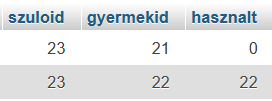
\includegraphics[width=5cm]{kepek/szulogyermek}
 	\caption{A 'szulogyermek' tábla részlete}
 	\label{fig:szulogyermek}
 \end{figure}
   
 uzenetek: Ez a tábla felelős az üzenetek tárolásáért. Tartalmazza természetesen a feladó és a címzett azonosítóját, valamint egy 'csoport' nevű mezőt is, mely a feladó és a címzett adataiból áll össze. Erre a jobb kereshetőség miatt volt szükség. Az üzenet dátumát, valamint természetesen az üzenet szövegét is tartalmazza. Tárgy mezőt nem hoztam létre, mert gondolataim szerint ez inkább egy 'Az iskola és a szülő közleményei' felület lenne, amelyben a szövegből egyértelműen kiderül az üzenet tárgya. Minden üzenetnek van egy státusza, ezt a státuszt már sajnos nem volt időm kidolgozni, de az értelme az lenne, hogy ha még nem olvasta a címzett, akkor a megjelenítésben jobban ki lenne emelve, jelezvén, hogy ez még nem lett elolvasva.
\chapter{Problémák, és megoldásuk a fejlesztés során}
Ebben a fejezetben kifejtem, hogy az alkalmazás mely részénél futottam bele olyan problémákba, amit nem tudtam egyszerűen, könnyen átlépni. Először a probléma felmerülésének helyét, leírását adom meg, majd több megoldást kipróbálok, végül leírom miért pont az adott megoldás lett a tökéletes.
\chapter{Felhasználói dokumentáció}
Ebben a fejezetben a felhasználók számára, világosan, érthetően, képernyőképekkel illusztrálva írom le a program működésének minden olyan funkcióját, amire szükségük lehet az alkalmazás használata során.
\chapter{Továbbfejlesztési lehetőségek}
Szeretnék egy olyan rendszert megalkotni, ami már-már továbbfejleszthetetlen. De természetesen ilyen nem létezik, soha nem is fog. Minden programban vannak továbbfejlesztési lehetőségek.
\section{Külső fájl importálása}
Akár Excel, akár csv fájlt is fel lehetne tölteni, amit a program feldolgoz, és az adatokat a megfelelő helyekre tárolja el. Például ha egy diák év közben érkezik az iskolánkba, akkor a személyes adatait felvehetjük, nem tart sokáig, ám az előző intézményben szerzett korábbi jegyeire is szükségünk lenne. Ezeket egyesével nagyon sok idő lenne felvinni, és a hibázási lehetőség is nagyon nagy. Ekkor jön a következő gondolat, hogy akkor Exportálásra is lenne igény, így tényleg a diák összes adatát egy pillanat alatt lementhetjük, és a másik rendszerben pedig beimportálás után használhatjuk.\\
Természetesen minden év elején a sok új diákot, és a szüleit is könnyedén fel lehetne tölteni a rendszerbe, amennyiben egy megfelelően formázott dokumentum rendelkezésre áll a feltöltésre.
\section{Órarend}
Egy elektronikus naplóban kézenfekvő megoldás, ha az órarendet is már az alkalmazás készíti el. Ahhoz, hogy ezt el lehessen készíteni, szükség van a tanárok, az osztályok, és a tantermek rögzítésére. Természetesen nem megfeledkezve a tantárgyakról, ami minden osztály esetében más és más. Ezek az adatok az általam készített programokban természetesen megvannak, így már csak maga az órarend generálásra lenne hátra. Ennek a megalkotása viszont felérne egy újabb fél éves fejlesztési folyamattal.
\section{Házi feladatok}
Ugyanúgy, ahogyan a jelenlegi programban a dolgozatok meg vannak valósítva, meg lehet ugyanezt a házi feladatra is valósítani. A  tanár kiadja a feladatot online, és a diákok otthon megcsinálva, feltölthetik a naplóba, ahonnan a tanár letöltés, nyomtatás, és piros toll használata nélkül egyszerűen tudná ellenőrizni. 
\section{Szülői, orvosi igazolás feltöltése}
Megvalósítható az is, hogy a szülő maga írja meg a Szülői igazolást, amit elmenthet Igazolásként. Ezt az osztályfőnök látja, és ez alapján állítja a meglévő hiányzás státuszát a megfelelőre. Az orvosi igazolással hasonló a helyzet. Amint a diák vagy a szülő kézhez kapta a betegséget igazoló dokumentumot, akkor feltöltheti azt képként a rendszerbe.
\section{Üzenet státusza}
Ahogy korábban már leírtam, időm nem volt rá sajnos, de a felhasználók segítségére válna egy olyan funkció, hogy a beérkezett üzeneteket megjelölhetné az alkalmazás valami feltűnő módon, hogy ez az üzenet, bizony még nem lett elolvasva. Gondolok itt akár kerettel körbevenni, vagy az üzenet elejét félkövér betűkkel kiemelni. Akár plusz gombbal tényleges elolvasás nélkül is lehetne olvasottnak jelölni.
\chapter{Összefoglalás}
Ebbe a fejezetbe kerül a probléma ismételt leírása, valamint a megoldásával együtt egy következtetés levonás.
\begin{thebibliography}{}
	https://www.digitnaplo.hu/\\
	https://www.mozaik.info.hu/Homepage/Mozaportal/MPdigitalis.php?op=mozanaplo\\
	https://ekreta.hu/\\
	https://hu.wikipedia.org/wiki/WAMP\\
	https://matebalazs.hu/javascript.html\\
	https://thispersondoesnotexist.com/ \\
	https://codingislove.com/realtime-search-javascript/\\
	http://www.sulibolt.hu/asc\_ism.html
\end{thebibliography}
\end{document}